\documentclass[11pt]{amsbook}
\usepackage{../HBSuerDemir}
\begin{document}
    \hPage{b2p2/414}
    \section{GEOMETRIC AND PHYSICAL APPLICATIONS}
    \subsection{GEOMETRIC APPLICATION (Area of a surface): }
    Let S: F(x, y, z) = 0 be a surface over the region R
in xy-plane (i.e. R is the projection of S on xy-planes). Then
the area of S is
    \begin{equation*}
        \hAbs{S}=\iint_S \,d\sigma 
    \end{equation*}    
    and we have\\
    \begin{equation*}
        \iint_S \,d\sigma= \iint_R \sec \gamma \overline {\,dx \,dy}
    \end{equation*}    	
\begin {figure}[ htbp ]
\begin {center}
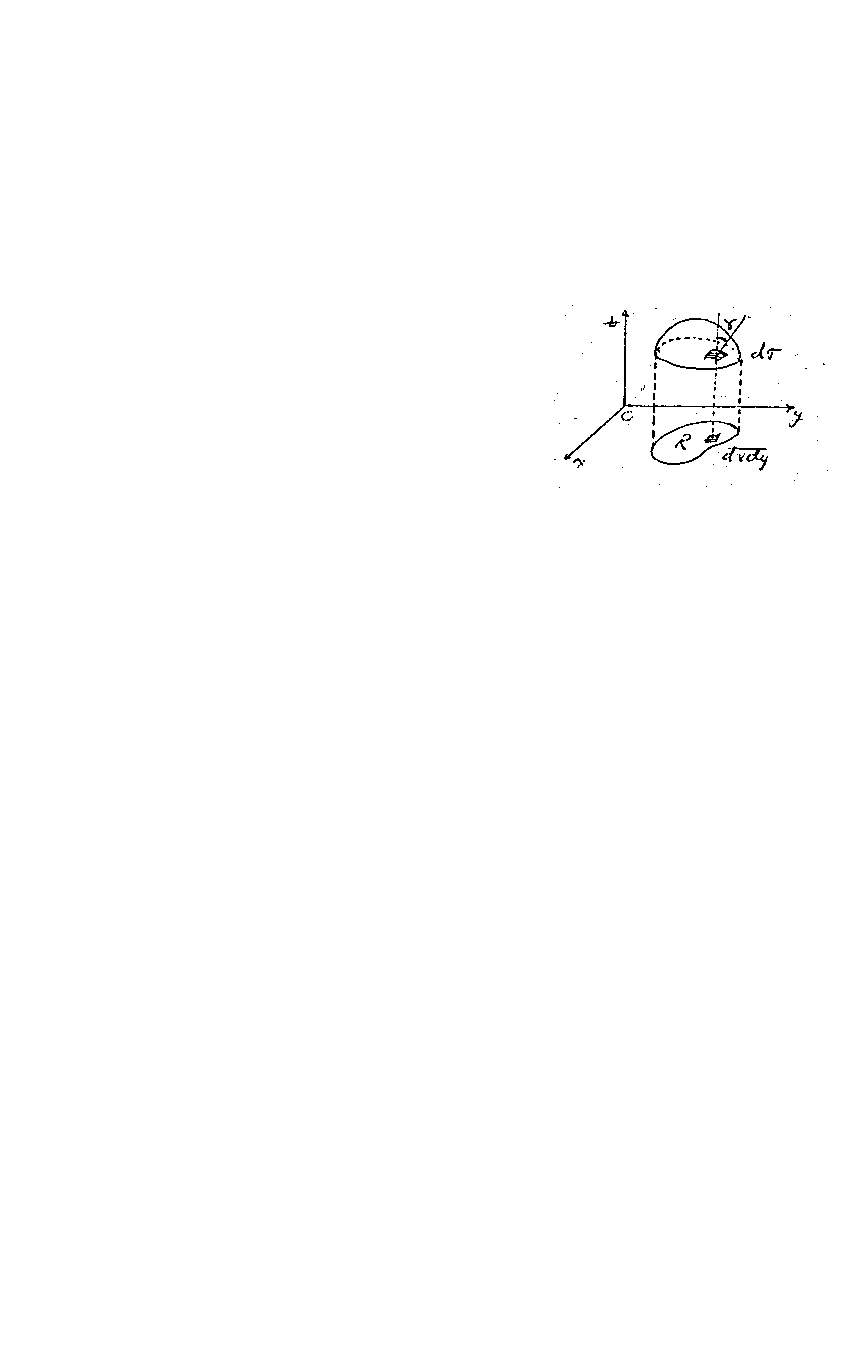
\includegraphics[width=0.4\columnwidth]{images/b2p1-130.pdf}


\label {fig: image}
\end{center}
\end{figure}

    where $d\sigma$ is the elementary area of S and y is the acute angle between the normal line to S at a point in $d\sigma$ and z-axis.\\
    Then,
    \begin{align*}       
    &\cos \gamma= \hAbs{\vec{n}.k}\\
    \Longrightarrow&\sec \gamma= \frac{1}{\hAbs{\vec{n}.k}}=
    \begin{cases}
        \sqrt{1+z_{x}^{2}+z_{y}^{2}}\quad if \quad z=f(x,y)\\
        \frac{\sqrt{F_{x}^{2}}+\sqrt{F_{y}^{2}}+\sqrt{F_{z}^{2}}}{\hAbs{F_{z}}}\quad if \quad f(x,y,z)=0
    \end{cases}
    \end{align*}

    

    and
    \begin{equation*}
        \hAbs{S}= \iint_R \sqrt{1+z_{x}^{2}+z_{y}^{2}}\ \overline {\,dx \,dy}\quad (or \iint_R \frac{\sqrt{F_{x}^{2}}+\sqrt{F_{y}^{2}}+\sqrt{F_{z}^{2}}}{\hAbs{F_{z}}}\ \overline {\,dx \,dy})
    \end{equation*}
    Similarly
        \begin{equation*}
        \hAbs{S}= \iint_R \sqrt{1+x_{x}^{2}+x_{z}^{2}}\ \overline {\,dx \,dz}\quad (or \iint_R \frac{\sqrt{F_{x}^{2}}+\sqrt{F_{y}^{2}}+\sqrt{F_{z}^{2}}}{\hAbs{F_{x}}}\ \overline {\,dy \,dz})
    \end{equation*}
        \begin{equation*}
        \hAbs{S}= \iint_R \sqrt{1+y_{x}^{2}+y_{z}^{2}}\ \overline {\,dx \,dz}\quad (or \iint_R \frac{\sqrt{F_{x}^{2}}+\sqrt{F_{y}^{2}}+\sqrt{F_{z}^{2}}}{\hAbs{F_{y}}}\ \overline {\,dx \,dz})
    \end{equation*}
    To obtain a simpler region R or a simpler integrand, one
projects S onto a convenient coordinate plane. 
\end{document}